% Chapter Template

\chapter{Results and Analysis} % Main chapter title

\label{c5} % Change X to a consecutive number; for referencing this chapter elsewhere, use \ref{ChapterX}

\section{Results and Discussion}


\begin{table*}[!ht]
  \centering
  \setlength{\tabcolsep}{3pt}
  {\renewcommand{\arraystretch}{1}%
  \caption{MAE performances of proposed models  and traditional models}
  \begin{tabular}{|l|c|c|c|c|c|p{0.15 \textwidth}|p{0.15\textwidth}|}
  \hline
  \textbf{MODEL} & \textbf{RNN} & \textbf{BILSTM} & \textbf{LSTM} & \textbf{GRU} & \textbf{CNN} &\textbf{Proposed1 \(\ GRU-BILSTM-LSTM \)\ } & \textbf{Proposed2 \(\ CNN-RNN\)\ } \\ \hline
  JODHPUR & 1.7717 & 1.7705 & 1.7314 & 1.7200 & 1.7390 & 1.7397 & 1.7857 \\ \hline
  AJMER & 1.7842 & 1.7497 & 1.7407 & 1.7324 & 1.7706 & 1.7617 & 1.8727 \\ \hline
  SOUTH DELHI & 2.0295 & 2.0003 & 1.9807 & 1.9665 & 2.0024 & 1.9888 & 2.0321 \\ \hline
  POKHRAN & 1.5997 & 1.6038 & 1.5830 & 1.5851 & 1.5925 & 1.6168 & 1.6261 \\ \hline
  BHUJ & 1.5547 & 1.4877 & 1.5013 & 1.4846 & 1.5000 & 1.4946 & 1.5728 \\ \hline
  BENGALURU & 14.0449 & 13.8617 & 13.7279 & 13.7272 & 13.7536 & 13.7506 & 14.3304 \\ \hline
  UDAIPUR & 1.7450 & 1.7447 & 1.7065 & 1.7080 & 1.7057 & 1.7089 & 1.8294 \\ \hline
  HYDERABAD & 1.5080 & 1.4934 & 1.4966 & 1.4941 & 1.5178 & 1.5174 & 1.5346 \\ \hline
  AHMEDABAD & 13.1670 & 12.9117 & 12.5405 & 12.6959 & 12.6091 & 12.6614 & 13.3079 \\ \hline
  AHMEDABAD2 & 1.7552 & 1.7141 & 1.7108 & 1.7015 & 1.7056 & 1.7245 & 1.8336 \\ \hline
  NEW DELHI & 2.0160 & 1.9922 & 1.9598 & 1.9443 & 1.9465 & 1.9541 & 1.9949 \\ \hline
  \label{mae}
  \end{tabular}%
  }
  \end{table*}
  The table above shows the MAE for various solar power generation forecasting models. These models were created using various DL architectures, each thoroughly evaluated for expected accuracy across various geographical regions represented by city names. The well-known designs explored in this study are RNN, BiLSTM, LSTM, GRU, and CNN. Furthermore, the evaluation contains two separate hybrid models, "Proposed1 (CNN-RNN)" and "Proposed1 (GRU-BILSTM-LSTM)". The MAE figures in the table indicate the average absolute difference between expected and actual solar power output. Smaller MAE values are essential since they are directly associated with higher predicted accuracy, proving the models' ability to reflect real-world data adequately. Individual models were seen at Jodhpur, Ajmer, South Delhi, Pokhran, Bhuj, Bengaluru, Udaipur, Hyderabad, Ahmedabad1, Ahmedabad2, and New Delhi. This tabular data allows for easy comparison of anticipated accuracy across geographic locations, allowing for the construction more effective models. Notably, the suggested hybrid models capitalise on the distinct features of their constituent designs, which may improve prediction accuracy. Finally, the graph displays the MAE levels of many DL algorithms that forecast solar power generation in various geographical regions.
  
  
  
  
  
  
  
  \begin{table*}[!ht]
  \centering
  \setlength{\tabcolsep}{3pt}
  {\renewcommand{\arraystretch}{1}%
  \caption{MSE performances of proposed models  and traditional models}
  \begin{tabular}{|l|c|c|c|c|c|p{0.15 \textwidth}|p{0.15\textwidth}|}
  \hline
  \textbf{MODEL} & \textbf{RNN} & \textbf{BILSTM} & \textbf{LSTM} & \textbf{GRU} & \textbf{CNN} &\textbf{Proposed1 \(\ GRU-BILSTM-LSTM \)\ } & \textbf{Proposed2 \(\ CNN-RNN\)\ } \\ \hline
  JODHPUR & 1.7736 & 1.7375 & 1.7375 & 1.7226 & 1.7340 & 1.7410 & 1.7764 \\ \hline
  AJMER & 1.7625 & 1.7591 & 1.7360 & 1.7189 & 1.7351 & 1.7514 & 1.8728 \\ \hline
  SOUTH DELHI & 1.9977 & 1.9833 & 1.9659 & 1.9485 & 1.9853 & 1.9811 & 2.0445 \\ \hline
  POKHRAN & 1.6037 & 1.6090 & 1.5857 & 1.5871 & 1.6069 & 1.6073 & 1.6435 \\ \hline
  BHUJ & 1.5260 & 1.4929 & 1.4902 & 1.4872 & 1.4945 & 1.4931 & 1.5585 \\ \hline
  BENGALURU & 14.1045 & 13.9399 & 13.7403 & 13.7480 & 13.7382 & 13.7518 & 14.3621 \\ \hline
  UDAIPUR & 1.7662 & 1.7273 & 1.7101 & 1.7022 & 1.7064 & 1.7129 & 1.7918 \\ \hline
  HYDERABAD & 1.5127 & 1.4944 & 1.4949 & 1.4865 & 1.5176 & 1.5121 & 1.5261 \\ \hline
  AHMEDABAD & 13.0194 & 12.8521 & 12.5125 & 12.6730 & 12.6556 & 12.8117 & 13.2173 \\ \hline
  AHMEDABAD2 & 1.7892 & 1.7190 & 1.7032 & 1.7091 & 1.7057 & 1.7156 & 1.8249 \\ \hline
  NEW DELHI & 2.0046 & 1.9909 & 1.9633 & 1.9459 & 1.9453 & 1.9501 & 1.9926 \\ \hline
  \label{MSE}
  \end{tabular}%
  }
  \end{table*}
  The MSE estimations for numerous solar power forecast models comprise many DL architectures evaluated for expected accuracy across various geographic locations represented by city names. DL architectures being considered include the RNN, BiLSTM, LSTM, GRU, CNN, and two proposed hybrid models, "Proposed1 (CNN-RNN)" and "Proposed2 (GRU-BILSTM-LSTM)". To show the model's performance in those locations, the table includes Jodhpur, Ajmer, South Delhi, Pokhran, Bhuj, Bengaluru, Udaipur, Hyderabad, Ahmedabad, Ahmedabad2, and New Delhi. This graph enables direct model accuracy comparison across locations, which aids in selecting more accurate models. By utilising the properties of their constituent architectures, the proposed hybrid models may improve projected accuracy. Finally, the table compares the MSE values of numerous DL models for predicting solar power in various locations. Examining these MSE values allows stakeholders to make educated choices regarding which models to use for accurate solar power estimation, as shown in Table \ref{MSE}.
  
  
  
  
  
  
  
  
  \begin{table*}[!ht]
  \centering
  \setlength{\tabcolsep}{3pt}
  {\renewcommand{\arraystretch}{1}%
  \caption{MAPE performances of proposed models  and traditional models}
  \begin{tabular}{|l|c|c|c|c|c|p{0.15 \textwidth}|p{0.15\textwidth}|}
  \hline
  \textbf{MODEL} & \textbf{RNN} & \textbf{BILSTM} & \textbf{LSTM} & \textbf{GRU} & \textbf{CNN} &\textbf{Proposed1 \(\ GRU-BILSTM-LSTM \)\ } & \textbf{Proposed2 \(\ CNN-RNN\)\ } \\ \hline
  JODHPUR & 1.7711 & 1.7498 & 1.7337 & 1.7169 & 1.7284 & 1.7486 & 1.7870 \\ \hline
  AJMER & 1.8117 & 1.7497 & 1.8397 & 1.8206 & 1.8140 & 1.8243 & 1.8824 \\ \hline
  SOUTH DELHI & 1.9996 & 1.9892 & 1.9629 & 1.9466 & 1.9706 & 1.9602 & 2.0027 \\ \hline
  POKHRAN & 1.6113 & 1.5960 & 1.5838 & 1.5793 & 1.5975 & 1.6236 & 1.6391 \\ \hline
  BHUJ & 2.4538 & 2.2615 & 6.2572 & 2.1085 & 10.1542 & 8.3704 & 2.5362 \\ \hline
  BENGALURU & 14.2304 & 13.9144 & 13.7414 & 13.7540 & 13.7466 & 13.7981 & 14.2304 \\ \hline
  UDAIPUR & 1.9100 & 1.7745 & 1.7536 & 1.7456 & 1.7405 & 1.7312 & 1.9138 \\ \hline
  HYDERABAD & 3.8611 & 1.9967 & 9.4425 & 1.8613 & 10.9414 & 2.7880 & 1.8110 \\ \hline
  AHMEDABAD & 25.3734 & 23.9855 & 83.9375 & 17.2330 & 102.6779 & 22.0346 & 17.1641 \\ \hline
  AHMEDABAD2 & 1.8833 & 1.7757 & 1.7434 & 1.7451 & 1.7455 & 1.7584 & 1.8523 \\ \hline
  NEW DELHI & 2.0076 & 1.9761 & 1.9582 & 1.9524 & 1.9411 & 1.9496 & 1.9898 \\ \hline
  \label{MAPE}
  \end{tabular}%
  }
  \end{table*}
  
  
  
  The table offers a comprehensive analysis of MAPE statistics for several models that predict solar output. It was determined how well the models in the table could predict outcomes across various geographic regions based on the names of the cities. RNN, GRU, CNN, BiLSTM, and LSTM are some of the DL models being studied. Two further suggested hybrid models, "Proposed1 (CNN-RNN)" and "Proposed2 (GRU-BILSTM-LSTM)", are also taken into account. The MAPE numbers in the table illustrate how well each model foresaw solar power in various cities. A lower MAPE score denotes higher solar power generation forecast accuracy. This study focused on several cities, including Jodhpur, Ajmer, South Delhi, Pokhran, Bhuj, Bengaluru, Udaipur, Hyderabad, Ahmedabad, Ahmedabad2, and New Delhi. The direct model performance comparison across several locations in this table may be used to determine whether models are more accurate in forecasting solar power generation. The recommended hybrid models were developed to use each component design's benefits, possibly increasing forecast accuracy. The accuracy with which various DL models predict solar energy output across various geographies is examined in depth in this table's conclusion. Stakeholders may choose which models will generate the most accurate projections of solar power by reviewing the MAPE values shown in the Teble \ref{MAPE}.
  
  
  
  
  
  
  
  
  
  
  
  \begin{table*}[!ht]
  \centering
  \setlength{\tabcolsep}{3pt}
  {\renewcommand{\arraystretch}{1}%
  \caption{RMSE performances of proposed models  and traditional models}
  \begin{tabular}{|l|c|c|c|c|c|p{0.15 \textwidth}|p{0.15\textwidth}|}
  \hline
  \textbf{MODEL} & \textbf{RNN} & \textbf{BILSTM} & \textbf{LSTM} & \textbf{GRU} & \textbf{CNN} &\textbf{Proposed1 \(\ GRU-BILSTM-LSTM \)\ } & \textbf{Proposed2 \(\ CNN-RNN\)\ } \\ \hline
  UDAIPUR & 1.7499 & 1.7484 & 1.7501 & 1.7267 & 1.731 & 1.8541 & 1.8512 \\ \hline
  NEW DELHI & 1.9072 & 1.9895 & 1.9718 & 1.9838 & 1.8936 & 2.0654 & 2.0509 \\ \hline
  BHUJ & 1.5179 & 1.5051 & 1.4948 & 1.5203 & 1.5317 & 1.6397 & 1.5676 \\ \hline
  BENGALURU & 14.2567 & 13.8596 & 13.9068 & 13.8904 & 14.1842 & 14.0226 & 14.4956 \\ \hline
  HYDERABAD & 1.5451 & 1.5392 & 1.5110 & 1.5074 & 1.5472 & 1.5617 & 1.5735 \\ \hline
  AHMEDABAD & 13.42 & 12.87 & 12.95 & 12.82 & 13.55 & 13.65 & 13.71 \\ \hline
  AHMEDABAD2 & 1.6990 & 1.6818 & 1.6982 & 1.7489 & 1.8299 & 1.8479 & 1.9134 \\ \hline
  POKHRAN & 1.6146 & 1.6274 & 1.6205 & 1.6114 & 1.6144 & 1.6446 & 1.6566 \\ \hline
  SOUTH DELHI & 2.0055 & 1.9952 & 1.9868 & 1.9981 & 2.0006 & 2.0304 & 2.0264 \\ \hline
  AJMER & 1.9246 & 1.8785 & 1.8642 & 1.8750 & 1.9282 & 1.9613 & 1.9647 \\ \hline
  JODHPUR & 1.7913 & 1.7589 & 1.7487 & 1.7542 & 1.7738 & 1.8431 & 1.8163 \\ \hline
  \label{RMSE}
  \end{tabular}%
  }
  \end{table*}
  
  The RMSE values for numerous forecasting models from diverse sectors are that each row represents a unique site, while the columns represent several solar power projection methods. In this study, RNN, BiLSTM, LSTM, GRU, CNN, and two proposed hybrid models, "Proposed1 (CNN-RNN)" and "Proposed2 (GRU-BILSTM-LSTM)", were all explored. The RMSE values for each model and location are displayed. Lower RMSE values imply better forecast accuracy. Notably, the proposed hybrid models outperform the component models in performance. The RMSE values for "Proposed1" in the "Udaipur" region, for example, are 1.8541 and 1.8512 for "Proposed2," with individual model RMSE values ranging from 1.7267 to 1.7501. According to the data in the table, the suggested hybrid models can improve forecasting accuracy, implying that solar power estimation may be used in various applications shown in Table \ref{RMSE}.
  
  
  
  \begin{figure}[!ht]
  \centering
  \includegraphics[width=\textwidth]{1act vs pred}
  \caption{Actual test data and proposed predictions of test data}
  \label{Line plot11}
  \end{figure}
  
  \begin{figure}[!ht]
  \centering
  \includegraphics[width=\textwidth]{2act vs pred}
  \caption{Actual test data and proposed predictions of test data for remaining cities}
  \label{Line plot11}
  \end{figure}
  
  
  
  
  
  \begin{figure*}[!ht]
  \centering
  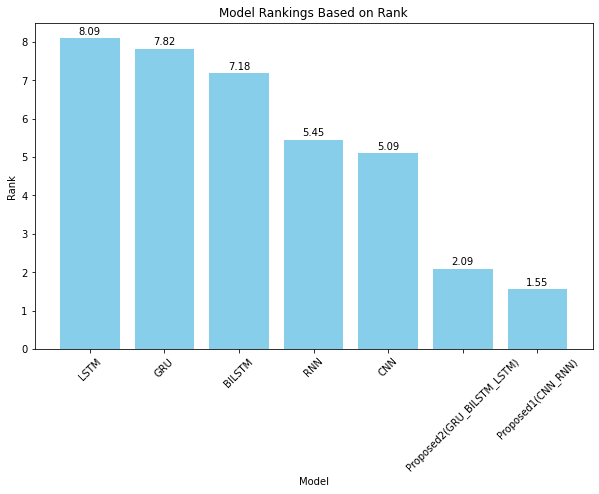
\includegraphics[width=\textwidth]{friedman ranking}
  \caption{Friedman ranking of proposed models and traditional DL models}
  \label{Line plot12}
  \end{figure*}
  
  
  
  
  
  
  